\documentclass{beamer}

\usepackage[utf8]{inputenc}
\usepackage[T1]{fontenc}

\usepackage{amssymb}
\usepackage{amsmath}
\usepackage{caption}
\usepackage{subcaption}
\usepackage{minted}
\usepackage{forest}
\usepackage{tabu}
\usepackage{pgfpages}


% Highlight boxes
\def\highlightbox#1{\setlength{\fboxsep}{2pt}\colorbox{yellow!60}{\textbf{#1}}}

\usetheme{Warsaw}
\useoutertheme{infolines}
\setbeamersize{text margin left=2em,text margin right=2em}

\makeatletter
\setbeamertemplate{footline}
{
  \leavevmode%
  \hbox{%
  \begin{beamercolorbox}[wd=.2\paperwidth,ht=2.25ex,dp=1ex,center]{author in head/foot}%
    \usebeamerfont{author in head/foot}\insertshortauthor%~~\beamer@ifempty{\insertshortinstitute}{}{(\insertshortinstitute)}
  \end{beamercolorbox}%
  \begin{beamercolorbox}[wd=.6\paperwidth,ht=2.25ex,dp=1ex,center]{title in head/foot}%
    \usebeamerfont{title in head/foot}\insertshorttitle
  \end{beamercolorbox}%
  \begin{beamercolorbox}[wd=.2\paperwidth,ht=2.25ex,dp=1ex,right]{date in head/foot}%
    \usebeamerfont{date in head/foot}\insertshortdate{}\hspace*{2em}
    \insertframenumber{} / \inserttotalframenumber\hspace*{2ex} 
  \end{beamercolorbox}}%
  \vskip0pt%
}
\makeatother

\begin{document}

\title{Optimizing NN Inference on Embedded Devices}
\subtitle{\vspace{0.8em}\small Master's Internship -- May-July 2018\\Snips Paris -- Under the supervision of Mathieu Poumeyrol}
\author{\vspace{0.5em}\\ Romain Liautaud\vspace{-2em}}
\date{}
\institute{\textit{École Normale Supérieure de Lyon}\\\vspace{-3em}}

{
\setbeamertemplate{headline}{}
\setbeamertemplate{navigation symbols}{}
\setbeamertemplate{footline}{}
\frame{\titlepage}
}

\frame{\frametitle{Overview}\tableofcontents} 

\section{Introduction}

\begin{frame}{About Snips}
\begin{center}
    \includegraphics[width=.3\textwidth]{snips-logo.png}
\end{center}

Snips is a french artificial intelligence startup which makes voice assistants (like Alexa or Siri), but with two specific goals:
\begin{itemize}
    \item Every assistant is \textbf{fully customizable}, from the choice of hotword to the intents that it recognizes.
    \item Every assistant is \textbf{private by design}, i.e. all queries that you ask to the assistant are never sent to a remote server (so all the computation must be done on device).
\end{itemize}
\vspace{2em}
\end{frame}

\begin{frame}{Deep Neural Networks at Snips}
\centering
\vspace{1em}
\includegraphics[width=.9\textwidth]{snips-pipeline.pdf}
\end{frame}

\begin{frame}{The problem}
    \begin{block}{}
    \textit{Neural networks are used everywhere in voice assistants, and they must run on device (e.g. Raspberry Pi or smartphones).}
    \end{block}
    
    \bigskip
    These devices have several limitations:
    \begin{itemize}
        \item Size of the inference runtime;
        \item Size of the stored trained models;
        \item Limited computational resources;
        \item Limited battery life;
        \item Special instruction set (ARMv7, ARMv8).
    \end{itemize}
\end{frame}

\begin{frame}{About my internship}
So traditional neural network libraries (e.g. TensorFlow, Theano, PyTorch, etc.) don't work well on these environments.\\

\note{Explain why.}

Several attempts at building specialized libraries:
\begin{itemize}
    \item TensorFlow Lite;
    \item XLA (ahead-of-time or just-in-time);
    \item TFDeploy, by the Snips Device Engineering team.\\ Written in Rust, a novel systems programming language.
\end{itemize}

\bigskip
During this internship, I had to find ways to improve TFDeploy w.r.t. speed, robustness, and space- and energy-efficiency.
\end{frame}

\begin{frame}{Representing a neural network: dataflow graphs}
TFDeploy is compatible with a subset of TensorFlow, so it borrows its internal representation of neural networks: \textbf{dataflow graphs}.

\vspace{1em}
Here on a basic perceptron:
\hspace*{-1.7em}
\includegraphics[width=1.1\textwidth]{example-perceptron.pdf}

\vspace{.5em}
\small
Each node has an \textit{operation}, a set of input and output \textit{ports} and a set of \textit{attributes}. Edges go from output port of a node to input port of another.

\note{
Before we begin:
\begin{itemize}
    \item The process was more engineering than research;
    \item Focus less on formalism and more on intuition.
\end{itemize}
}
\end{frame}

\section{Profiling and visualization tools}

\begin{frame}[fragile]{Profiling and visualization tools}
Command-line profiler:
\begin{exampleblock}{}
\footnotesize
\begin{minted}{bash}
cargo run -- ../../models/classic.pb -s 41x40xf32 profile
\end{minted}
\end{exampleblock}

\note{Issues with measuring precise values because of how small they are.}

\bigskip
Graph visualizer:
\begin{exampleblock}{}
\footnotesize
\begin{minted}{bash}
cargo run -- ../../models/classic.pb -s 41x40xf32 analyse --web
\end{minted}
\end{exampleblock}

\note{Custom-built layout with linear programming.}

\small{\textit{Without hints about the input shape:}}
\begin{exampleblock}{}
\footnotesize
\begin{minted}{bash}
cargo run -- ../../models/classic.pb analyse --web
\end{minted}
\end{exampleblock}
\end{frame}

\section{Static analysis of dataflow graphs}

\begin{frame}{Problem statement}
I first had to formalize and implement a \textbf{static analyser} for dataflow graphs (using ideas from abstract interpretation). Why?

\begin{itemize}
    \item To clarify TFDeploy error messages;
    \item To catch as many errors as possible before runtime;
    \item To get hints about the edge shapes for the visualizer;
    \item To build optimizations, e.g. constant propagation and folding.
\end{itemize}

\bigskip
Essentially, we want to tag each edge of the graph with invariants about the tensors that flow through it. For instance:
\begin{itemize}
    \item<1-> Every tensor flowing through this edge has datatype \texttt{float32};
    \item<2-> Every tensor flowing through this edge has the same value of $t$;
    \item<3-> Every tensor flowing through this edge has rank $2$ or more, and its first dimension is $5$.
\end{itemize}
\end{frame}

\begin{frame}{Formalism: type, value and shape facts}
\small
\begin{definition}
A \textbf{datatype fact} $f \in \mathcal{TF}$ is either:
\begin{itemize}
    \setlength\itemsep{0em}
    \item $\top_\mathcal{TF}$, which matches any possible datatype;
    \item $Only_\mathcal{TF}(T)$ for $T$ a datatype, which only matches a specific datatype;
    \item $\bot_\mathcal{TF}$, which signifies an error.
\end{itemize}
\end{definition}

\begin{definition}
A \textbf{value fact} $f \in \mathcal{VF}$ is either:
\begin{itemize}
    \setlength\itemsep{0em}
    \item $\top_\mathcal{VF}$, which matches any possible tensor;
    \item $Only_\mathcal{VF}(t)$ for $t$ a tensor, which only matches a specific tensor;
    \item $\bot_\mathcal{VF}$, which signifies an error.
\end{itemize}
\end{definition}
\end{frame}

\begin{frame}{Formalism: type, value and shape facts}
\small
\begin{definition}
A \textbf{shape fact} is an element of $\mathcal{SF} \equiv \{0,\ 1\} \times \left(\mathbb{N} \cup \{\_\}\right)^*$. The first element defines whether the shape is \textit{closed} or \textit{open}, and the second element is a sequence of either an integer~--~which matches a specific dimension~--~or ``$\_$''~--~which matches any dimension.
\end{definition}

\vspace{.5em}
A few examples:
\begin{itemize}
    \setlength\itemsep{0em}
    \item<1-> ``Every tensor has shape $(2, 2)$'': \texttt{[2, 2]};
    \item<2-> ``Every tensor has rank $2$'': \texttt{[\_, \_]};
    \item<3-> ``Every tensor has rank $\geq 2$ and first dimension $5$'': \texttt{[5, \_, ..]}.
\end{itemize}

\vspace{.5em}
\uncover<4->
{\begin{definition}
A \textbf{tensor fact} is an element of $\mathcal{F} \equiv \mathcal{TF} \times \mathcal{SF} \times \mathcal{VF}$.
\end{definition}}
\end{frame}

\begin{frame}{Formalism: Lattice structure and unification}
    \small
    From top to bottom: largest (least general) to smallest (most general).

    \vspace{2em}
    \scriptsize
    \begin{minipage}{.5\linewidth}
        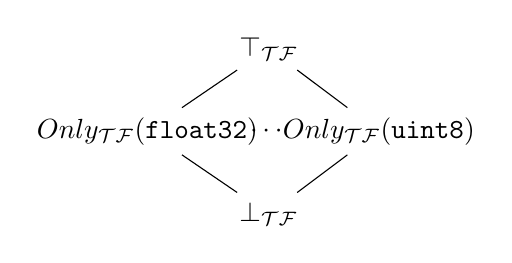
\begin{tikzpicture}[scale=0.7]
          \node (top) at (0,0) {$\top_\mathcal{TF}$};
          \node (a) at (-2.2,-1.5) {$Only_\mathcal{TF}(\texttt{float32})$};
          \node (dots) at (0,-1.5) {$\cdots$};
          \node (d) at (2,-1.5) {$Only_\mathcal{TF}(\texttt{uint8})$};
          \node (bot) at (0,-3) {$\bot_\mathcal{TF}$};
          \draw (top) -- (a) -- (bot) -- (d) -- (top);
        \end{tikzpicture}
    \end{minipage}%
    \begin{minipage}{.5\linewidth}
        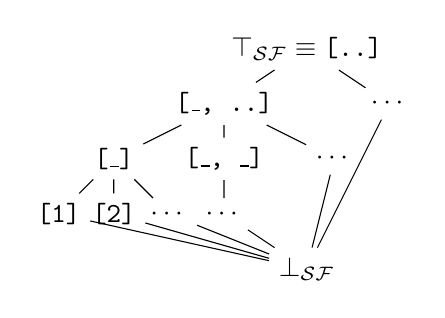
\begin{tikzpicture}[scale=0.7]
          \node (top) at (0,0) {$\top_\mathcal{SF} \equiv \texttt{[..]}$};
          \node (a1) at (-1.5,-1) {\texttt{[\_, ..]}};
          \node (ad) at (1.5,-1) {$\cdots$};
          \node (b1) at (-3.5,-2) {\texttt{[\_]}};
          \node (b2) at (-1.5,-2) {\texttt{[\_, \_]}};
          \node (bd) at (0.5,-2) {$\cdots$};
          \node (c1) at (-4.5,-3) {\texttt{[1]}};
          \node (c2) at (-3.5,-3) {\texttt{[2]}};
          \node (cd) at (-2.5,-3) {$\cdots$};
          \node (ed) at (-1.5, -3) {$\cdots$};
          \node (bot) at (0,-4) {$\bot_\mathcal{SF}$};
    
          \draw (a1) -- (top) -- (ad);
          \draw (b1) -- (a1) -- (b2);
          \draw (bd) -- (a1);
          \draw (c1) -- (b1) -- (c2);
          \draw (cd) -- (b1);
          \draw (ed) -- (b2);
         
          \draw (ad) -- (bot) -- (bd);
          \draw (cd) -- (bot) -- (ed);
          \draw (c1) -- (bot) -- (c2);
        \end{tikzpicture}
    \end{minipage}

    \begin{definition}
    \small
    For a lattice $L$, the \textbf{unification} of $a, b \in L$, written as $a \sqcap_L b$, is the largest $c \in L$ such that $c \sqsubseteq_L a$ and $c \sqsubseteq_L b$, i.e. the \textit{most general fact that combines the information from $a$ and $b$}. It can be $\bot_L$ if $a$ and $b$ are incompatible facts.
    \end{definition}
\end{frame}

\begin{frame}{Graph level: propagation algorithm}
    \textit{Basic example of execution:}
    \vspace{1em}
    
    \centering
    \only<+>{\hspace*{-3.5em}\includegraphics[scale=.7]{example-propagation-0.pdf}}
    \only<+>{\hspace*{-5em}\includegraphics[scale=.7]{example-propagation-1.pdf}}
    \only<+>{\hspace*{-4em}\includegraphics[scale=.7]{example-propagation-2.pdf}}
    \only<+>{\hspace*{-4em}\includegraphics[scale=.7]{example-propagation-3.pdf}}
    \only<+>{\hspace*{-1em}\includegraphics[scale=.7]{example-propagation-4.pdf}}
    \only<+>{\hspace*{-1em}\includegraphics[scale=.7]{example-propagation-5.pdf}}
    \only<+>{\hspace*{0em}\includegraphics[scale=.7]{example-propagation-6.pdf}}
    \only<+>{\hspace*{0em}\includegraphics[scale=.7]{example-propagation-7.pdf}}
    \only<+>{\hspace*{0em}\includegraphics[scale=.7]{example-propagation-8.pdf}}

    \note<1>{\begin{itemize}
    \item Start with the source graph.
    \item Compute an execution plan.
    \item Tag each edge with general facts.
    \item Each operator has an $enrich_{op}$ function which takes facts about the input and output tensors and gives more precise facts. Example of $enrich_\texttt{ExpandDims}$ : if we know the output data shape and the index, we can deduce the input data shape.
    \end{itemize}}
\end{frame}

\begin{frame}[fragile]{Operation level: declarative constraint solver}
    \begin{block}{}
    How do we easily (and generically) express the $enrich_{op}$ function?
    \end{block}
    \vspace{.5em}
    \scriptsize
    
    \note{Trickier than it seems to get this to type-check (proxies and casting etc.).}
    \begin{minted}{rust}
fn rules(&self, inputs, outputs) { // For the Pad operation.
    let (input, paddings, output) = (&inputs[0], &inputs[1], &outputs[0]);
    solver
        .equals(&inputs.len, 2)
        .equals(&outputs.len, 1)
        .equals(&output.datatype, &input.datatype)
        .equals(&paddings.datatype, DataType::DT_INT32)
        .equals(&input.rank, &output.rank)
        .equals(&paddings.rank, 2)
        .equals(&paddings.shape[0], &input.rank)
        .equals(&paddings.shape[1], 2)
        .given(&input.rank, move |solver, rank: usize| {
            (0..rank).for_each(|i| {
                solver.equals_zero(wrap!(
                    (-1, &output.shape[i]),      (1, &input.shape[i]),
                    (1,  &paddings.value[i][0]), (1, &paddings.value[i][1])));
            })
        });
}
    \end{minted}
\end{frame}

\begin{frame}{An example of optimization: constant folding}
    \small
    
    \begin{block}{}
    To save space and prevent useless runtime computations, we can pre-compute constant parts of the graph and store the result instead.
    \end{block}
    \vspace{1em}
    
    \only<1>{
        \textit{Sometimes it makes sense:}
        \hspace*{-2em}
        \includegraphics[width=1.1\textwidth]{constant-propagation.pdf}
    }
    
    \only<2>{
        \textit{Sometimes it doesn't:}
        \hspace*{-2em}
        \includegraphics[width=1.1\textwidth]{no-constant-propagation.pdf}
    }
\end{frame}

\section{New streaming semantics for dataflow graphs}

\begin{frame}{The issue with real-time data}
    \small
    
    \begin{block}{}
        How do you feed real-time data (e.g. samples from a microphone) to a neural network which expects a \texttt{[$N$, $K$]}-shaped tensor as an input?
    \end{block}
    
    $$I_i =
    \begin{pmatrix}
        s_i \\
        s_{i + 1} \\
        \cdots \\
        s_{i + N - 1}
    \end{pmatrix} \in M_{N, K}(\mathbb{R})
    $$
    
    \begin{itemize}
        \item Naïve method: feed a new $I_i$ every time a new sample is recorded;\\ \textit{(But samples overlap, so useless computations).}
        \note{Example of convolution the board.}
        \item Batched method: feed a new $I_i$ every $N$ new samples; \\ \textit{(But introduces latency and reduces accuracy).}
        \item Ideally, feed each new sample to the network separately. \\ \textit{(But not supported by traditional semantics of inference.)}
    \end{itemize}
\end{frame}

\begin{frame}{New streaming semantics}
    \small

    \begin{block}{}
        So we define new semantics for dealing with real-time data.
    \end{block}

    \begin{itemize}
        \item<1-> Every input of the network (i.e. \texttt{Placeholder} node) can have a \textbf{streaming dimension}. This information is propagated to the rest of the graph using the analyser.
        \item<2-> Instead of thinking about tensors, we think about \textbf{chunks} (which have size $1$ along the streaming dimension);
        \item<3-> Each operation is associated with a new \textbf{streaming evaluation function} which takes a chunk from one of the ports and might return a new chunk, and \textit{remembers data from previous iterations} using \textbf{buffers}:
        $$step_{op} \ :\ \mathcal{P}(\mathcal{A}_{op})\ \times \ \mathcal{B}_{op} \times \llbracket 0,\ n_i \llbracket \times (\{\bot\} \cup \mathbb{N}) \times \mathcal{T} \ \rightarrow  \mathcal{B}_{op} \times (\{\bot\} \cup \mathcal{T}^{n_o})$$
    \end{itemize}
\end{frame}


\begin{frame}{Streaming inference algorithm}
    \textit{Example of execution on the board:}
    \vspace{1em}
    \begin{center}
        \includegraphics[width=.8\textwidth]{example-streaming.pdf}
    \end{center}
    
    \note{\begin{itemize}
        \item Pre-compute constant parts of the graph.
        \item Compute execution order.
        \item Propagate chunks.
    \end{itemize}}
\end{frame}

\section{Convolution implementations on embedded devices}

\begin{frame}{How do we implement fast convolution?}
\small
\begin{block}{}
    2-D convolution \textit{(actually cross-correlation)} is usually the most time consuming operation during CNN inference.
\end{block}

\bigskip
\footnotesize
\note{Example on the board for every case.}
So the implementation matters:
\begin{itemize}
    \item \textbf{Naïve approach}: slide the filter and perform every matrix product separately;
    \item \textbf{Im2col} approach: single matrix product of two well-built matrices:\\
    \includegraphics[width=.8\textwidth]{im2col.png}\\
    \textit{(Courtesy of Leonardo Araujo dos Santos.)}
    \item \textbf{Im2col} approach with optimized GEMM \textit{(e.g. from GotoBLAS or BLIS)};
    \item \textbf{FFT}-based approaches: $f \times g = \mathcal{F}^{-1}\left(\mathcal{F}(f) \cdot \mathcal{F}(g)\right)$
\end{itemize}

\end{frame}

\section{Conclusion}

\begin{frame}{Conclusion}
\small
During this internship, I improved the speed, space- and energy-efficiency and robustness of TFDeploy via optimizations built on top of a static analyser for dataflow graphs; via new inference semantics for streaming data; and via a careful choice of the convolution implementation.\\

I also learned to tame Rust, and got a sense of how it feels doing research and implementation in a production environment.\\

Possible future improvements:
\begin{itemize}
    \item Make the declarative rule solver more expressive;
    \item Improve the performance of static analysis;
    \item Reduce the overhead on streaming evaluation;
    \item Custom implementation of im2col-based convolution to better control memory usage and speed.
\end{itemize}
\end{frame}

\end{document}